



METADATA

e.g.
tei:teiHeader
title, author, responsible for the edition, description of the source, encoding
=> Metadata of the file
tei:front
title page with the title, author, year of imprint (metadata from the source)
introduction (of the editor)


Spezialfälle der TEI, die relevant sein könnten:

titlePage
msDesc
sourceDesc 

Übung: Header ausfüllen













%---------------------------------
%OAIS: Open Archival Information System Reference Model
%OAI-PMH: Protocol for Metadata Harvesting
%GAMS: a digital archive for long-term preservation and repository


%---------------------------------


1945: Die Idee des Hypertextes
1986: SGML ISO Standard
1989: HTML von Tim Berners-Lee (CERN)
1994: W3C gegründet
1998: XML 1.0
1999: XSLT
2001: XML-Schema

%---------------------------------

%TODO Open Refine
% Metadata, Data Enrichment, Open Refine/Normdatenanreicherung / allg Normdaten, GND etc


%---------------------------------------------
\begin{frame}{FRBR (Functional Requirements for
Bibliographic Records)}

\bg{w3schools}{white}{Werk} Idee des Werks \\
Intellektuelle oder künstlerische Schöpfung

\bg{w3schools}{white}{Expression} Realisierung / Konkretisierung der Idee \\
e.g. bei einem Musikstück der Umstand, wie man ein Stück (Werkidee) spielt. Kann sehr unterschiedlich sein 
Form, die ein Werk annimmt, wenn es realisiert wird (e.g. in unterschiedlichen Sprachen).
Manifestiert wird es nur, wenn es e.g. mitgeschnitten wird.

Realisierung dieser Schöpfung, jenseits ihrer
physischen "Zufälligkeiten"

\bg{w3schools}{white}{Manifestation} physische Realisierung (e.g. als Buch, als Audiobuch, als CD, etc.) \\
\bg{w3schools}{white}{Item/Exemplar} Ein konkretes Ding der Manifestationsformen. Im Grunde identische Kopie des physischen Objektes.
Gesamtheit von identischen Verkörperungen

Attribute, Properties oder Prädikate können für jede Ebene einzeln definiert werden. e.g. Werkidee kann keine Sprache haben, Expression aber schon. 

Physisches Objekt
\end{frame}

%----------------------------------

\begin{frame}{Computer processable information}
    

Damit Daten automatisiert von Computern verarbeitet werden können, müssen wir sie
strukturieren.
\begin{itemize}
\item Ein Beispiel dafür ist XML, das wir im Kurs erlernen. Es basiert - wie auch das verwandte
HTML- auf SGML. (Im Unterschied zu HTML ist XML eben extensible, d.h. man kann seine
eigenen Elemente erfinden, was bei HTML nicht der Sinn der Sache ist).
\item XHTML ist HTML, das der XML-Struktur folgt.
XML
\item ist eine Meta-Syntax, mit der man andere Texte beschreiben kann.
\item ist ein Subset von SGML, das aber mehr als nur Text beschreiben kann (auch zB Bilder,
Musik, RDF).
\end{itemize}
Damit die Daten untereinander austauschbar werden (und auch Zeit und Energie bei der Wahl
passender Kodierungsschemata gespart werden kann), gibt es XML-Standards.
Ein sehr bekannter ist die TEI (Text Encoding Initiative), die zum De-Facto-Standard in den
Geisteswissenschaften geworden ist.Wiederholung: XML
●
●
●
●
●
XML $\to$ Datenstandard zur Speicherung und zum Austausch von Daten, der menschen- und
maschinenlesbar ist.
Wohlgeformtheit (Syntax, “Vokabular”), Validität (nach Schema, Semantik, “Grammatik”).
Speicherung unabhängig vom Ausgabe-/Präsentationsmedium (single source
Prinzip/Publishing)
XML liefert Syntax; das Schema die zu verwendenden Elemente und wie sie eben zu verwenden
sind. Es gibt Schemasprachen zur Beschreibung dieser Schemata, z.B. DTD und XMLSchema;
Bsp. in der Einheit: Dublin Core.
XML-Standards/TEI: Man muss das nicht alles auswendig können, sondern schaut Elemente
immer nach Bedarf nach, weil sie sehr ausführlich definiert sind. Wie XML generell funktioniert,
sollte man wissen (und lernt es auch schnell). Dieses Wissen gilt unabhängig von den Schemata
und kann für jedes Schema weiterverwendet werden.Wiederholung: XML
Wir merken uns:
1.
2.
3.
Russische Puppen (Verschachtelung, kein
overlapping markup erlaubt, falls nötig gibt es aber
Behelfslösungen dafür)
Doppelkeks (Starttag-Inhalt-Endtag)
Baumstruktur (mit nur 1 Wurzelknoten/-element =
root).Schemata
Maintenance Helfer, um Redundanz und Inkonsistenz zu vermeiden, d.h. eigentlich eine Art
Hilfstool für das praktische Arbeiten, da wichtig wird, sobald die Anzahl der verwendeten Elemente,
Attribute und Attributwerte zu groß wird, als dass man leicht den Überblick verlieren könnte oder z.B. sehr
viele Leute am Projekt beteiligt sind, aber ggf. alle mit wenig Stunden (zB Studienassistenz), sodass die
Einzelnen nie so tief in der Materie sind, dass sie da noch durchsteigen würden bzw das realistisch
möglich ist, dass sie das noch können, ohne Inkonsistenzen einzubauen. Hier helfen ODD und Schemata,
weil sie eben nur erlaubte und dem Schema entsprechende Strukturen zulassen.Was bisher getan wurde\dots
\end{frame}
%---------------------------------------------
\begin{frame}{Trennung von Struktur und Darstellung}

\begin{itemize}
    \item Seit SGML ist ein wichtiges Prinzip die Trennung von Inhalt/Struktur und Darstellung
    \item vermeidet Redundanz, vgl. MS Word `Formatvorlagen': Ich kann das Aussehen des Gesamtdokuments schnell ändern, ohne jede Einzelinstanz umschreiben zu müssen. So auch bei \LaTeX{}, HTML, etc.
    \item der Fokus von XML auf die Beschreibung der Daten erlaubt das \emph{single-source}-Prinzip, d.h. ich kann aus einer Quelldatei, die alle Daten verdichtet enthält, mehrere -- ggf. weniger inhaltsreiche -- auf die Darstellung ausgerichtete Repräsentationen der / Ansichten auf die Daten erstellen (durch eine XSL-Transformation z.B. nach HTML für Webseiten oder \LaTeX{} für den Druck)
\end{itemize}

\end{frame}


%-----------------------------------------------------
\begin{frame}{XML: eXtensible Markup Language}
\metroset{block=fill}
\begin{columns}
\column{0.45\textwidth}
\footnotesize
\begin{itemize}
    \item deskriptiv $\neq$ prozedural \item erweiterbar (nicht wie bei HTML): kein fixiertes Tag-Set \item UTF-8 kodiert
    \item \bg{alert}{white}{Bedeutung der Daten > Darstellung}
     \item expliziert Implizites oder eine Interpretation \item Hinzufügen von (Meta-)Information \item maschinelle Weiterverarbeitung 
     \item Standard für Beschreibung und Austausch von Daten 
     \item \bg{alert}{white}{universelle Metasprache}
\end{itemize}
\column{0.45\textwidth}
\footnotesize
\begin{block}{}
\bg{w3schools}{white}{Nachteile}~  `geschwätzig', Overlapping-Problem, langsam verglichen mit JSON und relationalen Datenbanken -- hat aber auch Features, die die nicht haben (\& für GeWi sehr wichtig sind)
\medskip

\bg{w3schools}{white}{menschen- und maschinenlesbar}~ 
\medskip

{unabhängig von Ausgabeformat}~ (Papier, Bildschirm)
\end{block}
\end{columns}


\end{frame}



%----------------------------------
\begin{frame}[allowframebreaks]{TEI Basics}
\footnotesize
TEI = \bg{alert}{white}{modular} $\to$ im Schema können Untermengen festgelegt werden (`Ich benutze Core und \dots ') \item \href{http://www.tei-c.org/Roma/}{ROMA Schema} \item sonst TEI P5 All
\smallskip

\bg{w3schools}{white}{Gemeinsamkeiten von Textdokumenten: } \\
\bg{alert}{white}{\href{http://www.tei-c.org/release/doc/tei-p5-doc/en/html/CO.html}{TEI Core} }

\begin{itemize}\footnotesize
    \item Identifikatoren (Seitenangaben, Signatur, Inventarnummer, Regalnummer, etc.)
    \item Abschnitte und Unterabschnitte (Gliederung)
    \item Abbildungen, Skizzen, grafische Elemente
    \item Schreibmodus (Prosa, Drama, Vers etc.)
    \item Strukturelle Einheiten (Absatz, Listen, Strophen, Zeilen, Reden, etc.)
    \item Textunterschiede oftmals durch unterschiedliche Formatierung gekennzeichnet (Titel, Überschriften, Zitate, Betonungen, etc.)
    \item Sachinformationen (Personen, Orte, etc.)
    \item Texteingriffe Korrekturen, Streichungen, Revisionen
\end{itemize}
\vspace{1em}

\bg{w3schools}{white}{Warum TEI verwenden oder nicht?} \\
\textbf{Nachteil:} man muss Regeln befolgen -- muss man aber sonst sinnvollerweise eh auch. Wollte man es wirklich gut machen, wäre es viel Arbeit! Andererseits: Flexibilität. TEI hat nicht immer etwas für Spezialzwecke. \\
\textbf{Vorteil:} die Regeln hat sich schon jemand überlegt, man muss sie nur nachschauen, verstehen und anwenden. Allgemeiner Standard in den Geisteswissenschaften, macht Daten unterschiedlicher Projekte interoperabel.
\end{frame}




%-----------------------------------------------------
\begin{frame}{\texttt{<msDesc>}}
$\to$ \href{http://gams.uni-graz.at/o:corema.b1/sdef:TEI/get?mode=view:msdesc}{Example: CoReMA (Cooking Recipes of the Middle Ages)}

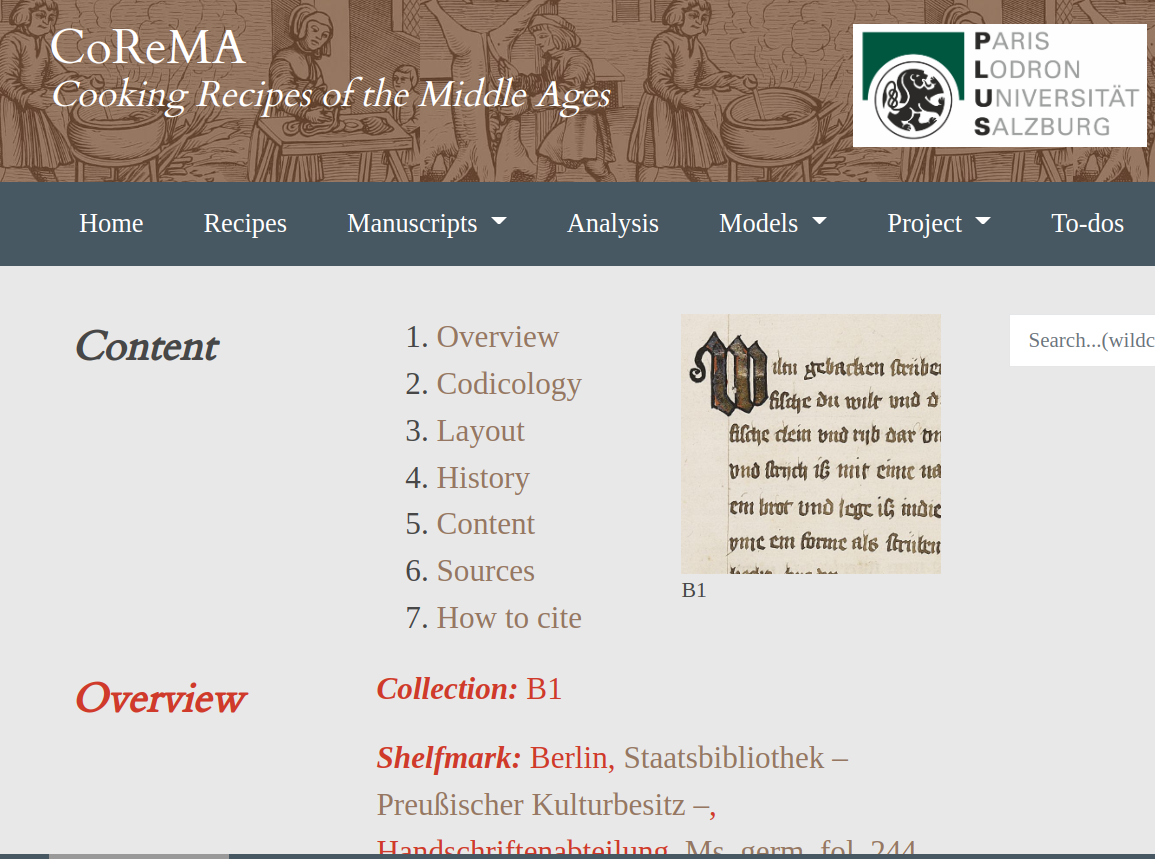
\includegraphics[width=0.75\textwidth]{img/corema-msDesc.png}

\end{frame}

\begin{frame}[allowframebreaks,fragile]{\texttt{<msDesc>}}

\begin{xmlcode}
<TEI xmlns="http://www.tei-c.org/ns/1.0">
  <teiHeader>
    <fileDesc>
      <titleStmt>
        <title>Electronic transcription of Berlin, Staatsbibliothek 
        zu Berlin – Preußischer Kulturbesitz –, 
        Handschriftenabteilung; Ms. germ. fol. 244 </title>
      </titleStmt>
      <editionStmt> [...] </editionStmt>
      <publicationStmt>
        <publisher>
          <ref target="https://informationsmodellierung.uni-graz.at"></ref>
          <orgName ref="http://d-nb.info/gnd/1137284463">
          ZIM-ACDH, Universität Graz</orgName>
        </publisher>
        <authority>
          <ref target="https://informationsmodellierung.uni-graz.at"></ref>
          <orgName ref="http://d-nb.info/gnd/1137284463">
          Zentrum für Informationsmodellierung - Austrian Centre 
          for Digital Humanities, Karl-Franzens-Universität Graz</orgName>
        </authority>
        <distributor>
          <ref target="https://gams.uni-graz.at"></ref>
          <orgName>GAMS - Geisteswissenschaftliches 
          Asset Management System</orgName>
        </distributor>
        [...]
\end{xmlcode}


\framebreak 


\begin{xmlcode}
[...]
        <availability>
          <licence n="text" target="https://creativecommons.org/licenses/by/4.0">
          Creative Commons BY 4.0</licence>
          <licence n="facsimile" target="https://creativecommons.org/licenses/by-nc-sa/4.0/">
          Creative Commons BY-NC-SA 4.0 </licence>
        </availability>
        <date when="2020-01-01"></date>
        <pubPlace>Graz</pubPlace>
        <idno type="PID">o:corema.b1</idno>
        <ref target="info:fedora/context:corema" type="context"></ref>
        <ref target="info:fedora/context:corema.glyph" type="context"></ref>
      </publicationStmt>
      <sourceDesc>
        <msDesc>
          <msIdentifier>
            <country>Deutschland</country>
            <settlement>Berlin</settlement>
            <institution ref="https://staatsbibliothek-berlin.de/">Staatsbibliothek – Preußischer Kulturbesitz –</institution>
            <repository>Handschriftenabteilung</repository>
            <idno ref="https://digital.staatsbibliothek-berlin.de/werkansicht?PPN=PPN785884734&amp;PHYSID=PHYS_0001&amp;DMDID=">Ms. germ. fol. 244 </idno>
            <altIdentifier type="abbr">
              <idno>B1</idno>
            </altIdentifier>
          </msIdentifier>
          [...]
\end{xmlcode}


\framebreak 


\begin{xmlcode}
[...]
          <msContents>
            <textLang ana="manuscript">
              <lang ana="main" n="Q707007">Rhine Franconian</lang>
            </textLang>
          </msContents>
          <physDesc>
            <objectDesc form="composite-Manuscript">
              <supportDesc>
                <extent>
                  <measure type="leavesCount" unit="leaf">307</measure>
                  <dimensions type="block" unit="mm">
                    <height>370</height>
                    <width>260-270</width>
                  </dimensions>
                </extent>
                <foliation>
                  <ab type="completeness">7 ungezählte, leere Bll.;<lb></lb>
										Bll. 8+9 fehlen in der Zählung; ab 23r eigene alte Zählung</ab>
                </foliation>
                <collation>
                  <ab>Bll. 8+9 lose einliegend;<lb></lb>
										zw. 91 und 92 fehlt ein Bl.;<lb></lb>
										Bll. 131 und 142 vertauscht</ab>
                </collation>
                <condition> [...] </condition>
              </supportDesc>
              <layoutDesc>       
         <layout columns="1"> [...] </layout>
              </layoutDesc>
            </objectDesc>
            <handDesc hands="1">
              <handNote>Gesamte Handschrift in sorgfältiger <term>Textura</term> geschrieben.</handNote>
            </handDesc>
            <scriptDesc facs="fol. 285r-294v" resp="Astrid Böhm">
              <scriptNote>
                <desc>allgemeine Beobachtung</desc>
                <p>typische Textura, gebrochene Schrift, wenig Ligaturen</p>
              </scriptNote>
              <!-- many more scriptNotes -->
            </scriptDesc>
            
          </physDesc>
[...]
\end{xmlcode}



\framebreak 

\begin{xmlcode}
[...]
          <history>
            <origin>
              <origDate>
                <date notAfter="1450" notBefore="1440" xml:lang="de">ca. 1445</date>
                <date notAfter="1450" notBefore="1440" xml:lang="en">ca. 1445</date>
              </origDate>
              <origDate corresp="&apos;#012v">1447</origDate>
              <origDate corresp="&apos;#016v">1447</origDate>
              <origPlace>
                <placeName xml:lang="de">Gegend von Mainz</placeName>
                <placeName xml:lang="en">area of Mainz</placeName>: Aufgrund von Wasserzeichen, der rheinfränkischen Sprache und einem Kalender der Diözese Mainz dort verortet.</origPlace>
            </origin>
            <provenance>Vorbesitzer wohl ein Würzburger Mantiker und Astrologe.<lb></lb>
							Die Hs. wurde 1801 auf linksrheinischem Gebiet für die Pariser Nationalbibliothek konfisziert und kam nach dem Wiener Kongress 1815 an die Königliche Bibliothek Berlin.</provenance>
          </history>
          <msPart n="1r-6r">
            <msIdentifier>
              <idno>Astrologisch-mantisch-diätetische Sammlung</idno>
            </msIdentifier>
            <msContents>
              <textLang>
                <lang ana="main" n="Q707007">Rhine Franconian</lang>
              </textLang>
              <msItem corresp="#artes" xml:id="b1.1r-6r.1">
                <locus ana="folio">1r-6r</locus>
                <title>Planetenlehre</title>
              </msItem>
            </msContents>
          </msPart>
          [...]
\end{xmlcode}


\end{frame}





\section{The workshop}

\begin{frame}{Goals}
\subsection{Goals}
\begin{enumerate}
    \item get to know XPath \& XSLT (and learn how to use it)
    \item understand the role of XML/TEI, XPath and XSLT in Digital Editing
    \item be able to use XSLT to generate HTML and \LaTeX{} output from TEI
    \item \alert{Two days isn't enough for you to master XSLT!}
\end{enumerate}

\metroset{block=fill}
\begin{alertblock}{Schedule}
\footnotesize
\begin{description}
  \item[Day 1, morning] XML, TEI and Digital Editing $\to$ repetition of the basics, making sure we're all on the same page, understanding why we're even learning XSLT.
  \item[Day 1, afternoon] Navigating XML documents using XPath, introduction to HTML (\& Bootstrap) and \LaTeX{} (\& \texttt{reledmac})
  \item[Day 2] Transforming XML documents into HTML \& \LaTeX{} output formats using XSLT
\end{description}
\end{alertblock}
\end{frame}

\begin{frame}[standout]
    Single point of entry for all workshop-related materials: 
    \alert{\href{https://latex-ninja.com/2022/04/17/first-ever-latex-ninja-workshop-at-harvard-beyond-tei-digital-editions-with-xpath-and-xslt-for-the-web-and-in-latex/}{\LaTeX{} Ninja blogpost}} \& \alert{\href{https://github.com/sarahalang/Harvard_BeyondTEI_Workshop_SLang2022}{Github Repository}} (`additional resources' directory)
\end{frame}


\begin{frame}{Introductions}
\subsection{Introductions}
  \begin{columns}[T,onlytextwidth]
    \column{0.35\textwidth}
      \begin{alertblock}{Please introduce yourselves!}
      \footnotesize
        \begin{enumerate}
            \item Name, pronouns, field/topic of study
            \item Why did you come to this workshop?
            \item Previous experience with Digital Humanities (DH) or editing?
        \end{enumerate}
      \end{alertblock}

 \metroset{block=fill}
 { \setbeamersize{description width=1em}
      \begin{block}{Contact} 
      \begin{description}\scriptsize 
        \item[\faTwitter] \href{https://twitter.com/SarahALang_}{@SarahALang\_} \\ \href{https://twitter.com/latex_ninja}{@latex\_ninja}
        \item[\faHome] \protect\url{sarahalang.com} \\ \protect\url{latex-ninja.com}
        \item[\faAt] \protect\url{sarah.lang@uni-graz.at}
      \end{description}
      \end{block}
      }

    \column{0.6\textwidth}
      \metroset{block=fill}
      \begin{block}{Sarah Lang (she/they)}
      \scriptsize
      \begin{itemize}
          \item originally from Germany, now in Graz (Austria)
          \item Studied Latin, French \& History (teacher's education) in Graz \& Montpellier (France), then Archaeology Bachelor, Master in Religious Studies \& Philosophy
          \item got a DH certificate \& started working at Zentrum für Informationsmodellierung (ZIM) / Centre for Information Modelling in Graz
          
          \begin{itemize}\scriptsize
              \item Moral Weeklies/Spectators $\to$ \protect\url{gams.uni-graz.at/mws}
              \item Graz Repository of Ancient Fables (GRaF) $\to$ \protect\url{gams.uni-graz.at/graf}
              \item \emph{PhD thesis:} Decoding alchemical \emph{Decknamen} digitally. A Polysemantic Annotation and Machine Reasoning Algorithm for the Corpus of Iatrochymist Michael Maier (1568--1622)
          \end{itemize}
          \item \emph{Now:} teaching in Graz, Passau \& Vienna; PostDoc in Graz. \emph{Research interests:} history of science (alchemy), Neo-Latin, text mining and computer vision
      \end{itemize}
      \end{block}
  \end{columns}
\end{frame}

